\documentclass[a0paper,final,landscape]{baposter}
%\usepackage{times}
%\usepackage{calc}
%\usepackage{graphicx}
%\usepackage{amsmath}
%\usepackage{amssymb}
\usepackage{relsize}
\usepackage{varwidth}
%\usepackage{multirow}
%\usepackage{bm}
\usepackage{caption}
\usepackage{graphicx}
\usepackage{svg}
%\usepackage{multicol}
\usepackage{pst-node}
%\usepackage{blindtext}

\usepackage[utf8]{inputenc}
% \usepackage{fontspec}

\newfontfamily{\FA}{FontAwesome}

\usepackage{pgfplots}
\usetikzlibrary{matrix}
\usepgfplotslibrary{groupplots}
\pgfplotsset{compat=newest}
\usepackage{fontawesome}

\usepackage{pgfbaselayers}
\pgfdeclarelayer{background}
\pgfdeclarelayer{foreground}
\pgfsetlayers{background,main,foreground}

%\usepackage{helvet}
%\usepackage{bookman}
%\usepackage{palatino}
\usepackage{enumitem}
%\usepackage{wasysym}

\usepackage{amsmath,amsfonts,amsthm,amssymb}
\usepackage{mathtools}
\usepackage{siunitx}
\usepackage{fontawesome}
\usepackage{lmodern}
%\usepackage{chemmacros}
%\usepackage{authblk}

% \newcommand{\captionfont}{\footnotesize}

\selectcolormodel{cmyk}
\graphicspath{{images/}}

\captionsetup[figure]{font={sf, small}}

%%%%%%%%%%%%%%%%%%%%%%%%%%%%%%%%%%%%%%%%%%%%%%%%%%%%%%%%%%%%%%%%%%%%%%%%%%%%%%%%
%%%% Some math symbols used in the text
%%%%%%%%%%%%%%%%%%%%%%%%%%%%%%%%%%%%%%%%%%%%%%%%%%%%%%%%%%%%%%%%%%%%%%%%%%%%%%%%
% Format
\newcommand\myfrac[2]{\genfrac{}{}{0pt}{#1}{#2}}
\newcommand{\Matrix}[1]{\begin{bmatrix} #1 \end{bmatrix}}
\newcommand{\Vector}[1]{\Matrix{#1}}
\newcommand*{\SET}[1]  {\ensuremath{\mathcal{#1}}}
\newcommand*{\MAT}[1]  {\ensuremath{\mathbf{#1}}}
\newcommand*{\VEC}[1]  {\ensuremath{\bm{#1}}}
\newcommand*{\CONST}[1]{\ensuremath{\mathit{#1}}}
\newcommand*{\norm}[1]{\mathopen\| #1 \mathclose\|}% use instead of $\|x\|$
\newcommand*{\abs}[1]{\mathopen| #1 \mathclose|}% use instead of $\|x\|$
\newcommand*{\absLR}[1]{\left| #1 \right|}% use instead of $\|x\|$

\usepackage{xspace}
\newcommand{\id}{\ensuremath{1 \! \! \mathbb{I}}}
\newcommand{\eg}{e.g.,\xspace}
\newcommand{\Eg}{E.g.,\xspace}
\newcommand{\ie}{i.e.,\xspace}
\newcommand{\wo}{wo.\xspace}
\newcommand{\etal}{\emph{et al.}\xspace}
\newcommand{\cf}{cf.\xspace}
\newcommand{\invitro}{in vitro\xspace}
\newcommand{\Invitro}{In vitro\xspace}
\newcommand{\MP}{M$\Phi$\xspace}
\newcommand{\dd}{\ensuremath{\, \mathrm{d}}}

\newcommand{\lb}{\ensuremath{\left(}}
\newcommand{\rb}{\ensuremath{\right)}}
\newcommand{\lsb}{\ensuremath{\left[\,}}
\newcommand{\rsb}{\ensuremath{\, \right]}}
\newcommand{\BigOh}[1]{\ensuremath{\mathcal{O}(#1)}}

\newcommand{\nonlocalgrad}[1]{\ensuremath{\,\overset{\circ}{\nabla}_{#1}\;}}
\newcommand{\ngrad}{\ensuremath{\nonlocalgrad{R}}}
\def\norm#1{\mathopen\| #1 \mathclose\|}% use instead of $\|x\|$
\newcommand{\normLR}[1]{\left\| #1 \right\|}% use instead of $\|x\|$
\newcommand{\kraft}{\ensuremath{\boldsymbol{p}}}
\newcommand{\supp}{\mathop{\mathrm{supp}}}

\newcommand{\cinterval}[1]{\ensuremath{\left[#1\right]}}
\newcommand{\sgn}{\operatorname{sgn}}
\newcommand{\defeq}{\mathrel{\mathop:}=}
\newcommand{\eqdef}{\mathrel{\mathop=}:}

\theoremstyle{plain}
\newtheorem{lemma}{Lemma}

\theoremstyle{definition}
\newtheorem{definition}{Definition}

\definecolor{MidnightBlue}{cmyk}{0.78,0.78,0,0.56}
\definecolor{PiggyPink}{cmyk}{0, 0.7808, 0.4429, 0.1412}

%%%%%%%%%%%%%%%%%%%%%%%%%%%%%%%%%%%%%%%%%%%%%%%%%%%%%%%%%%%%%%%%%%%%%%%%%%%%%%%%
% Multicol Settings
%%%%%%%%%%%%%%%%%%%%%%%%%%%%%%%%%%%%%%%%%%%%%%%%%%%%%%%%%%%%%%%%%%%%%%%%%%%%%%%%
\setlength{\columnsep}{0.7em}
\setlength{\columnseprule}{0mm}

%%%%%%%%%%%%%%%%%%%%%%%%%%%%%%%%%%%%%%%%%%%%%%%%%%%%%%%%%%%%%%%%%%%%%%%%%%%%%%%%
% Save space in lists. Use this after the opening of the list
%%%%%%%%%%%%%%%%%%%%%%%%%%%%%%%%%%%%%%%%%%%%%%%%%%%%%%%%%%%%%%%%%%%%%%%%%%%%%%%%
\newcommand{\compresslist}{%
\setlength{\itemsep}{1pt}%
\setlength{\parskip}{0pt}%
\setlength{\parsep}{0pt}%
}

%%%%%%%%%%%%%%%%%%%%%%%%%%%%%%%%%%%%%%%%%%%%%%%%%%%%%%%%%%%%%%%%%%%%%%%%%%%%%%
%%% Begin of Document
%%%%%%%%%%%%%%%%%%%%%%%%%%%%%%%%%%%%%%%%%%%%%%%%%%%%%%%%%%%%%%%%%%%%%%%%%%%%%%
\newenvironment{flushenum}{%
 \begin{enumerate}[leftmargin=0.25cm,itemindent=.5cm,labelwidth=\itemindent,
         labelsep=0cm,align=left,itemsep=0em,parsep=0pt,topsep=0.1cm,label=\bfseries\arabic*.]
  \compresslist
  \setlength{\leftmargin}{0pt}
}{\end{enumerate}}

\newenvironment{flushitem}{%
\begin{itemize}[leftmargin=0.25cm,itemindent=.5cm,labelwidth=\itemindent,
labelsep=0cm,align=left,itemsep=0em,parsep=0pt]
  \compresslist
  \setlength{\leftmargin}{0pt}
}{\end{itemize}}

\def\twitter{{\small \FA \faTwitter}}
\def\home{{\small \FA \faHome}}
\def\homeLarge{{\huge \FA \faHome}}
\def\mail{{\small \FA \faEnvelopeAlt}}

\begin{document}

%%%%%%%%%%%%%%%%%%%%%%%%%%%%%%%%%%%%%%%%%%%%%%%%%%%%%%%%%%%%%%%%%%%%%%%%%%%%%%
%%% Here starts the poster
%%%---------------------------------------------------------------------------
%%% Format it to your taste with the options
%%%%%%%%%%%%%%%%%%%%%%%%%%%%%%%%%%%%%%%%%%%%%%%%%%%%%%%%%%%%%%%%%%%%%%%%%%%%%%
\typeout{Poster Starts}
% \background{
%   \begin{tikzpicture}[remember picture,overlay]%
%     \draw (current page.north west)+(-2em,-0em) node[anchor=north west] {\hspace{-2em}\includegraphics[height=1.1\textheight]{silhouettes_background}};
%   \end{tikzpicture}%
% }
%\definecolor{silver}{cmyk}{0,0,0,0.3}
% \definecolor{yellow}{cmyk}{0,0,0.9,0.0}
% \definecolor{reddishyellow}{cmyk}{0,0.22,1.0,0.0}
%\definecolor{black}{cmyk}{0,0,0.0,1.0}
% \definecolor{darkYellow}{cmyk}{0,0,1.0,0.5}
%\definecolor{darkSilver}{cmyk}{0,0,0,0.1}

\definecolor{UAgreen}{RGB}{0,124,65}
\definecolor{UAblack}{RGB}{0,0,0}
\definecolor{UAorange}{RGB}{255,160,35}
\definecolor{darkorange}{cmyk}{0.00,0.6,1.00,0.08}
\definecolor{lightgreen}{RGB}{210,255,210}
\definecolor{lightergreen}{RGB}{234,255,234}
\definecolor{lightestgreen}{cmyk}{0,0,0.05,0.0}

\begin{poster}{%
  % Show grid to help with alignment
  grid=false,
  columns=3,
  % Column spacing
  colspacing=1em,
  bgColorOne=white,
  % Background color for the gradient on the left side of the poster
  bgColorTwo=UAgreen,
  % Background color for the gradient on the right side of the right side
  borderColor=black, % Border color
  headerColorOne=MidnightBlue, % Background color for the header in the content
  % boxes l
  headerColorTwo=MidnightBlue, % Background color for the header in the content
  % boxes r
  headerFontColor=white, % Text color for the header text in the content
  % boxes
  % boxColorOne=lightestgreen, % Background color of the content boxes
  % boxColorTwo=lightestgreen,
  boxColorOne=white, % Background color of the content boxes
  boxColorTwo=white,
  % Format of textbox
  textborder=roundedleft,
  % Format of text header
  eyecatcher=true,
  headerborder=open,
  headerheight=0.12\textheight,
  headershape=roundedright,
  headershade=plain,
  headerfont=\large\bfseries\textsf, %Sans Serif
  boxshade=plain,
  background=shadeTB,
  linewidth=2.5pt
  }
  % Eye Catcher
  {%
  {\begin{minipage}{5em}
      
\includegraphics[height=6.5em]{ubc-logo-2018-crest-black-rgb300.png}
    \hfill
  \end{minipage}}
  } % No eye catcher for this poster. If an eye catcher is present, the title
  % is centered between eye-catcher and logo.
  % Title
  {\sf\huge\bfseries\centering %Sans Serif
  %\bf% Serif
    Fire-Climate Relationships in Continental Southeast Asia (SEA)
  }
  % Authors
  {\centering\sf %Sans Serif
  % Serif
  Vanessa Cheung,
  Alex Han,
  Danny Huang,
  Anthony Wu\hspace{3em}\\
  {\smaller
      Client: Andrea Ku, MSc Candidate at UBC Department of Geography\\
      Supervised by Professors Keegan Korthauer, Melissa Lee, Rodolfo Lourenzutti, and Chloe You from UBC Department of Statistics\\
  }
  }

  %\tikzstyle{light shaded}=[top color=baposterBGtwo!30!white,bottom color=baposterBGone!30!white,shading=axis,shading angle=30]

  % Width of left inset image

%%%%%%%%%%%%%%%%%%%%%%%%%%%%%%%%%%%%%%%%%%%%%%%%%%%%%%%%%%%%%%%%%%%%%%%%%%%%%%
%%% Now define the boxes that make up the poster
%%%---------------------------------------------------------------------------
%%% Each box has a name and can be placed absolutely or relatively.
%%% The only inconvenience is that you can only specify a relative position
%%% towards an already declared box. So if you have a box attached to the
%%% bottom, one to the top and a third one which should be in between, you
%%% have to specify the top and bottom boxes before you specify the middle
%%% box.
%%%%%%%%%%%%%%%%%%%%%%%%%%%%%%%%%%%%%%%%%%%%%%%%%%%%%%%%%%%%%%%%%%%%%%%%%%%%%%
%
% A coloured circle useful as a bullet with an adjustably strong filling
\newcommand{\colouredcircle}[1]{%
  \tikz{\useasboundingbox (-0.2em,-0.32em) rectangle(0.2em,0.32em);
\draw[draw=black,fill=baposterBGone!80!black!#1!white,line width=0.03em] (0,0)
circle(0.18em);}}

%%%%%%%%%%%%%%%%%%%%%%%%%%%%%%%%%%%%%%%%%%%%%%%%%%%%%%%%%%%%%%%%%%%%%%%%%%%%%%
\headerbox{Abstract}{name=introduction,column=0,row=0}{%
%%%%%%%%%%%%%%%%%%%%%%%%%%%%%%%%%%%%%%%%%%%%%%%%%%%%%%%%%%%%%%%%%%%%%%%%%%%%%%
{\fontfamily{lmss}\selectfont
Our project investigates relationships between climate factors (i.e. rainfall) and fire activity in continental SEA. We find that drought severity and percentage of vegetation have the greatest influence. Additionally, fire patterns do vary according to geographical patterns across SEA.
} 
}
%%%%%%%%%%%%%%%%%%%%%%%%%%%%%%%%%%%%%%%%%%%%%%%%%%%%%%%%%%%%%%%%%%%%%%%%%%%%%
%\headerbox{Objective}{name=objective,column=0,below=introduction}{\bfseries
%%
%Derive model~\eqref{Eqn:ArmstrongModel} from an underlying stochastic random
%walk.
%%
%}
%%%%%%%%%%%%%%%%%%%%%%%%%%%%%%%%%%%%%%%%%%%%%%%%%%%%%%%%%%%%%%%%%%%%%%%%%%%%%%
\headerbox{Introduction}{name=master,column=0,below=introduction}{%
%%%%%%%%%%%%%%%%%%%%%%%%%%%%%%%%%%%%%%%%%%%%%%%%%%%%%%%%%%%%%%%%%%%%%%%%%%

{\bf{\textsf{Research Questions}}}
{\fontfamily{lmss}\selectfont
\begin{flushenum}
    \item How do fire patterns vary across continental SEA?
    \item How do rainfall patterns influence the variations in fire activity?
\end{flushenum}
} 

{\bf{\textsf{Exploratory Data Analysis}}}
\vspace{-0.7em}
\begin{center}
    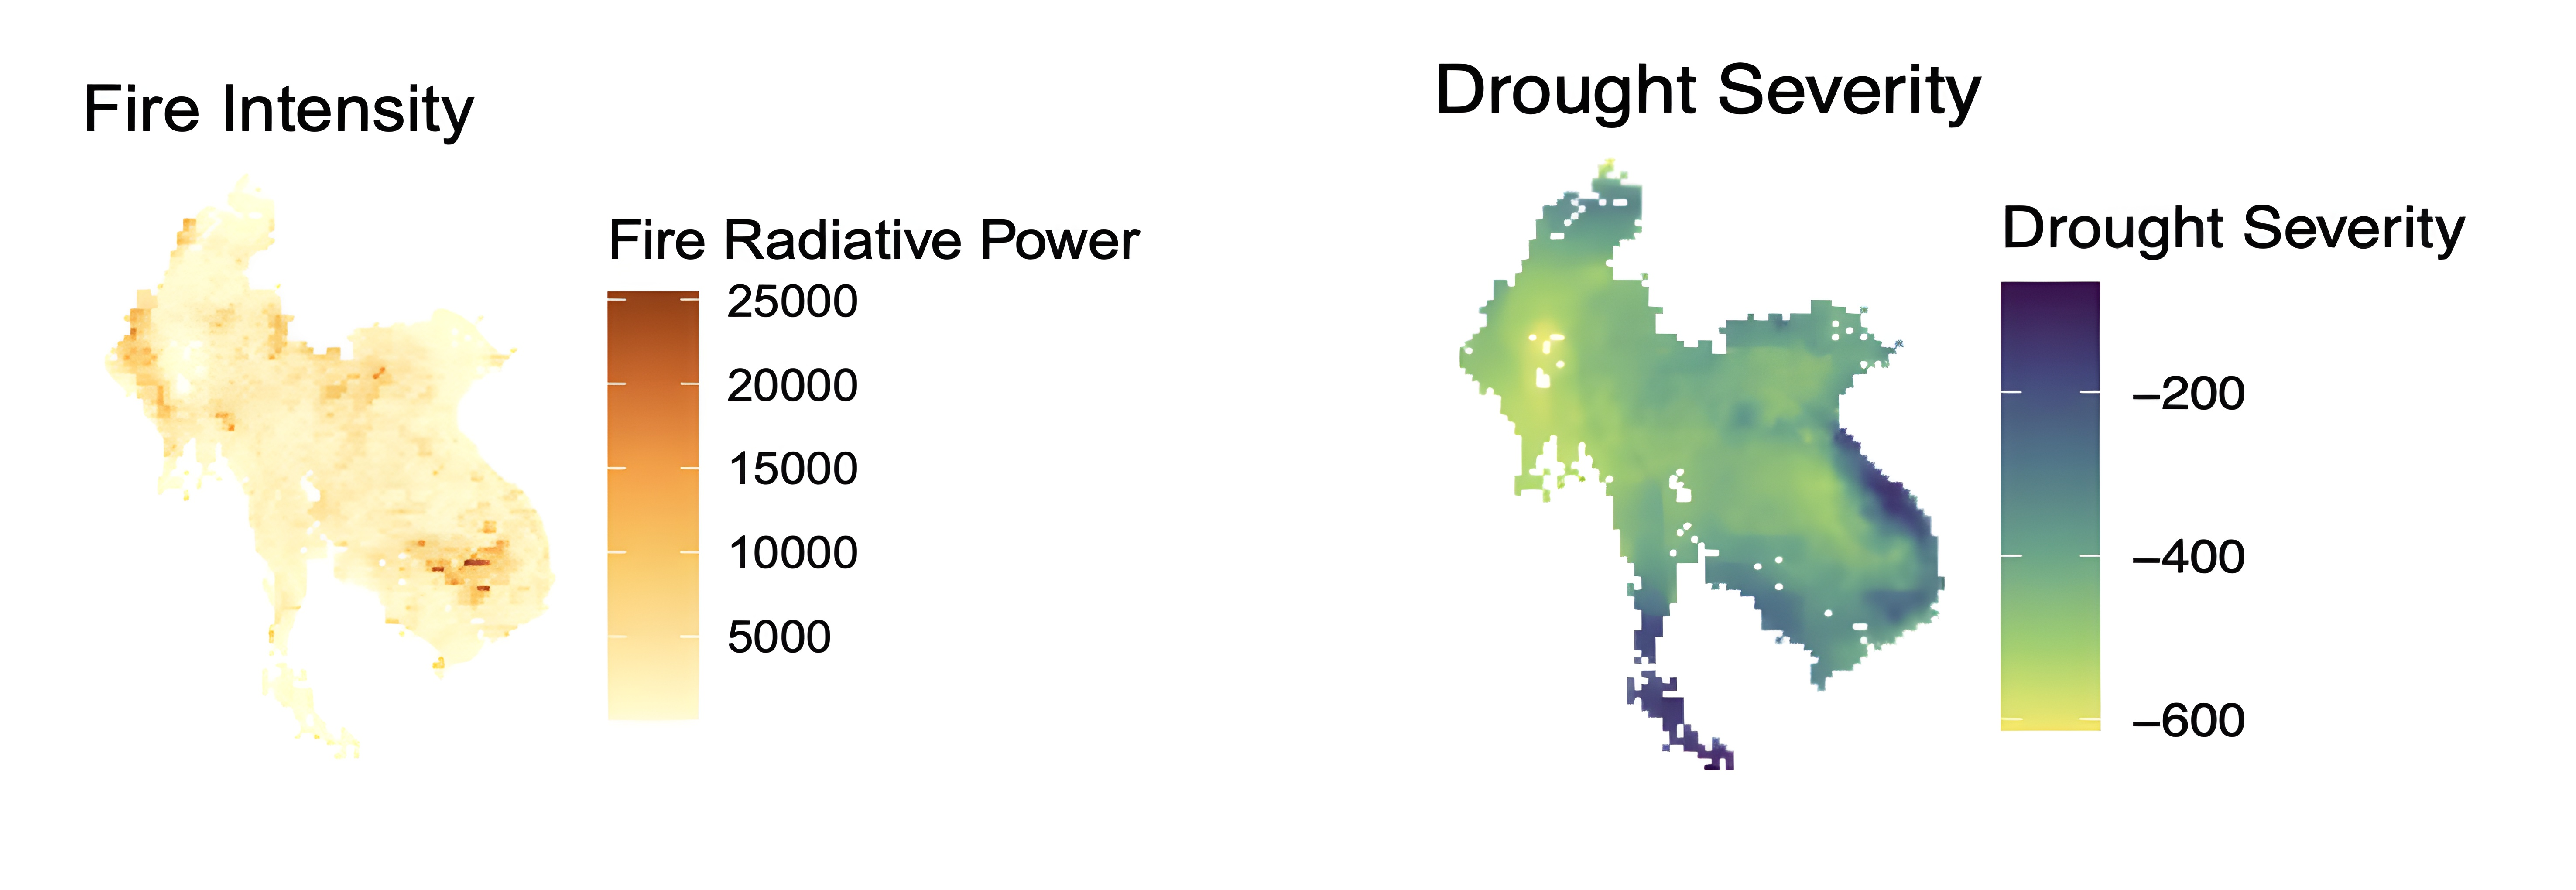
\includegraphics[width=\textwidth]{./images/HQ_EDA.png}
    \captionof{figure}{
    {\fontfamily{lmss}\selectfont
    Visualizing data by raster graphics.
    }
    }
\end{center}

{\bf{\textsf{Regionalization}}}
{\fontfamily{lmss}\selectfont
\vspace{-0.7em}
\begin{flushitem}
    \item Aim to cluster SEA into “similar” regions by fire patterns using Spatial 'K'luster Analysis by Tree Edge Removal (SKATER) algorithm.
\end{flushitem}
}

{\bf{\textsf{Statistical Analysis}}}
\vspace{-0.7em}
{\fontfamily{lmss}\selectfont
\begin{flushitem}
    \item Analyze model performance and variable importance by Generalized Additive Models (GAM) and Random Forest Regression (RF).
\end{flushitem}
}
}

%%%%%%%%%%%%%%%%%%%%%%%%%%%%%%%%%%%%%
\headerbox{Results on Regionalization}{name=derivation,column=0,span=1,below=master}{%
%%%%%%%%%%%%%%%%%%%%%%%%%%%%%%%%%%%%%%%%%%%%%%%%%%%%%%%%%%%%%%%%%%%%%%%%%%%%%%
\begin{center}
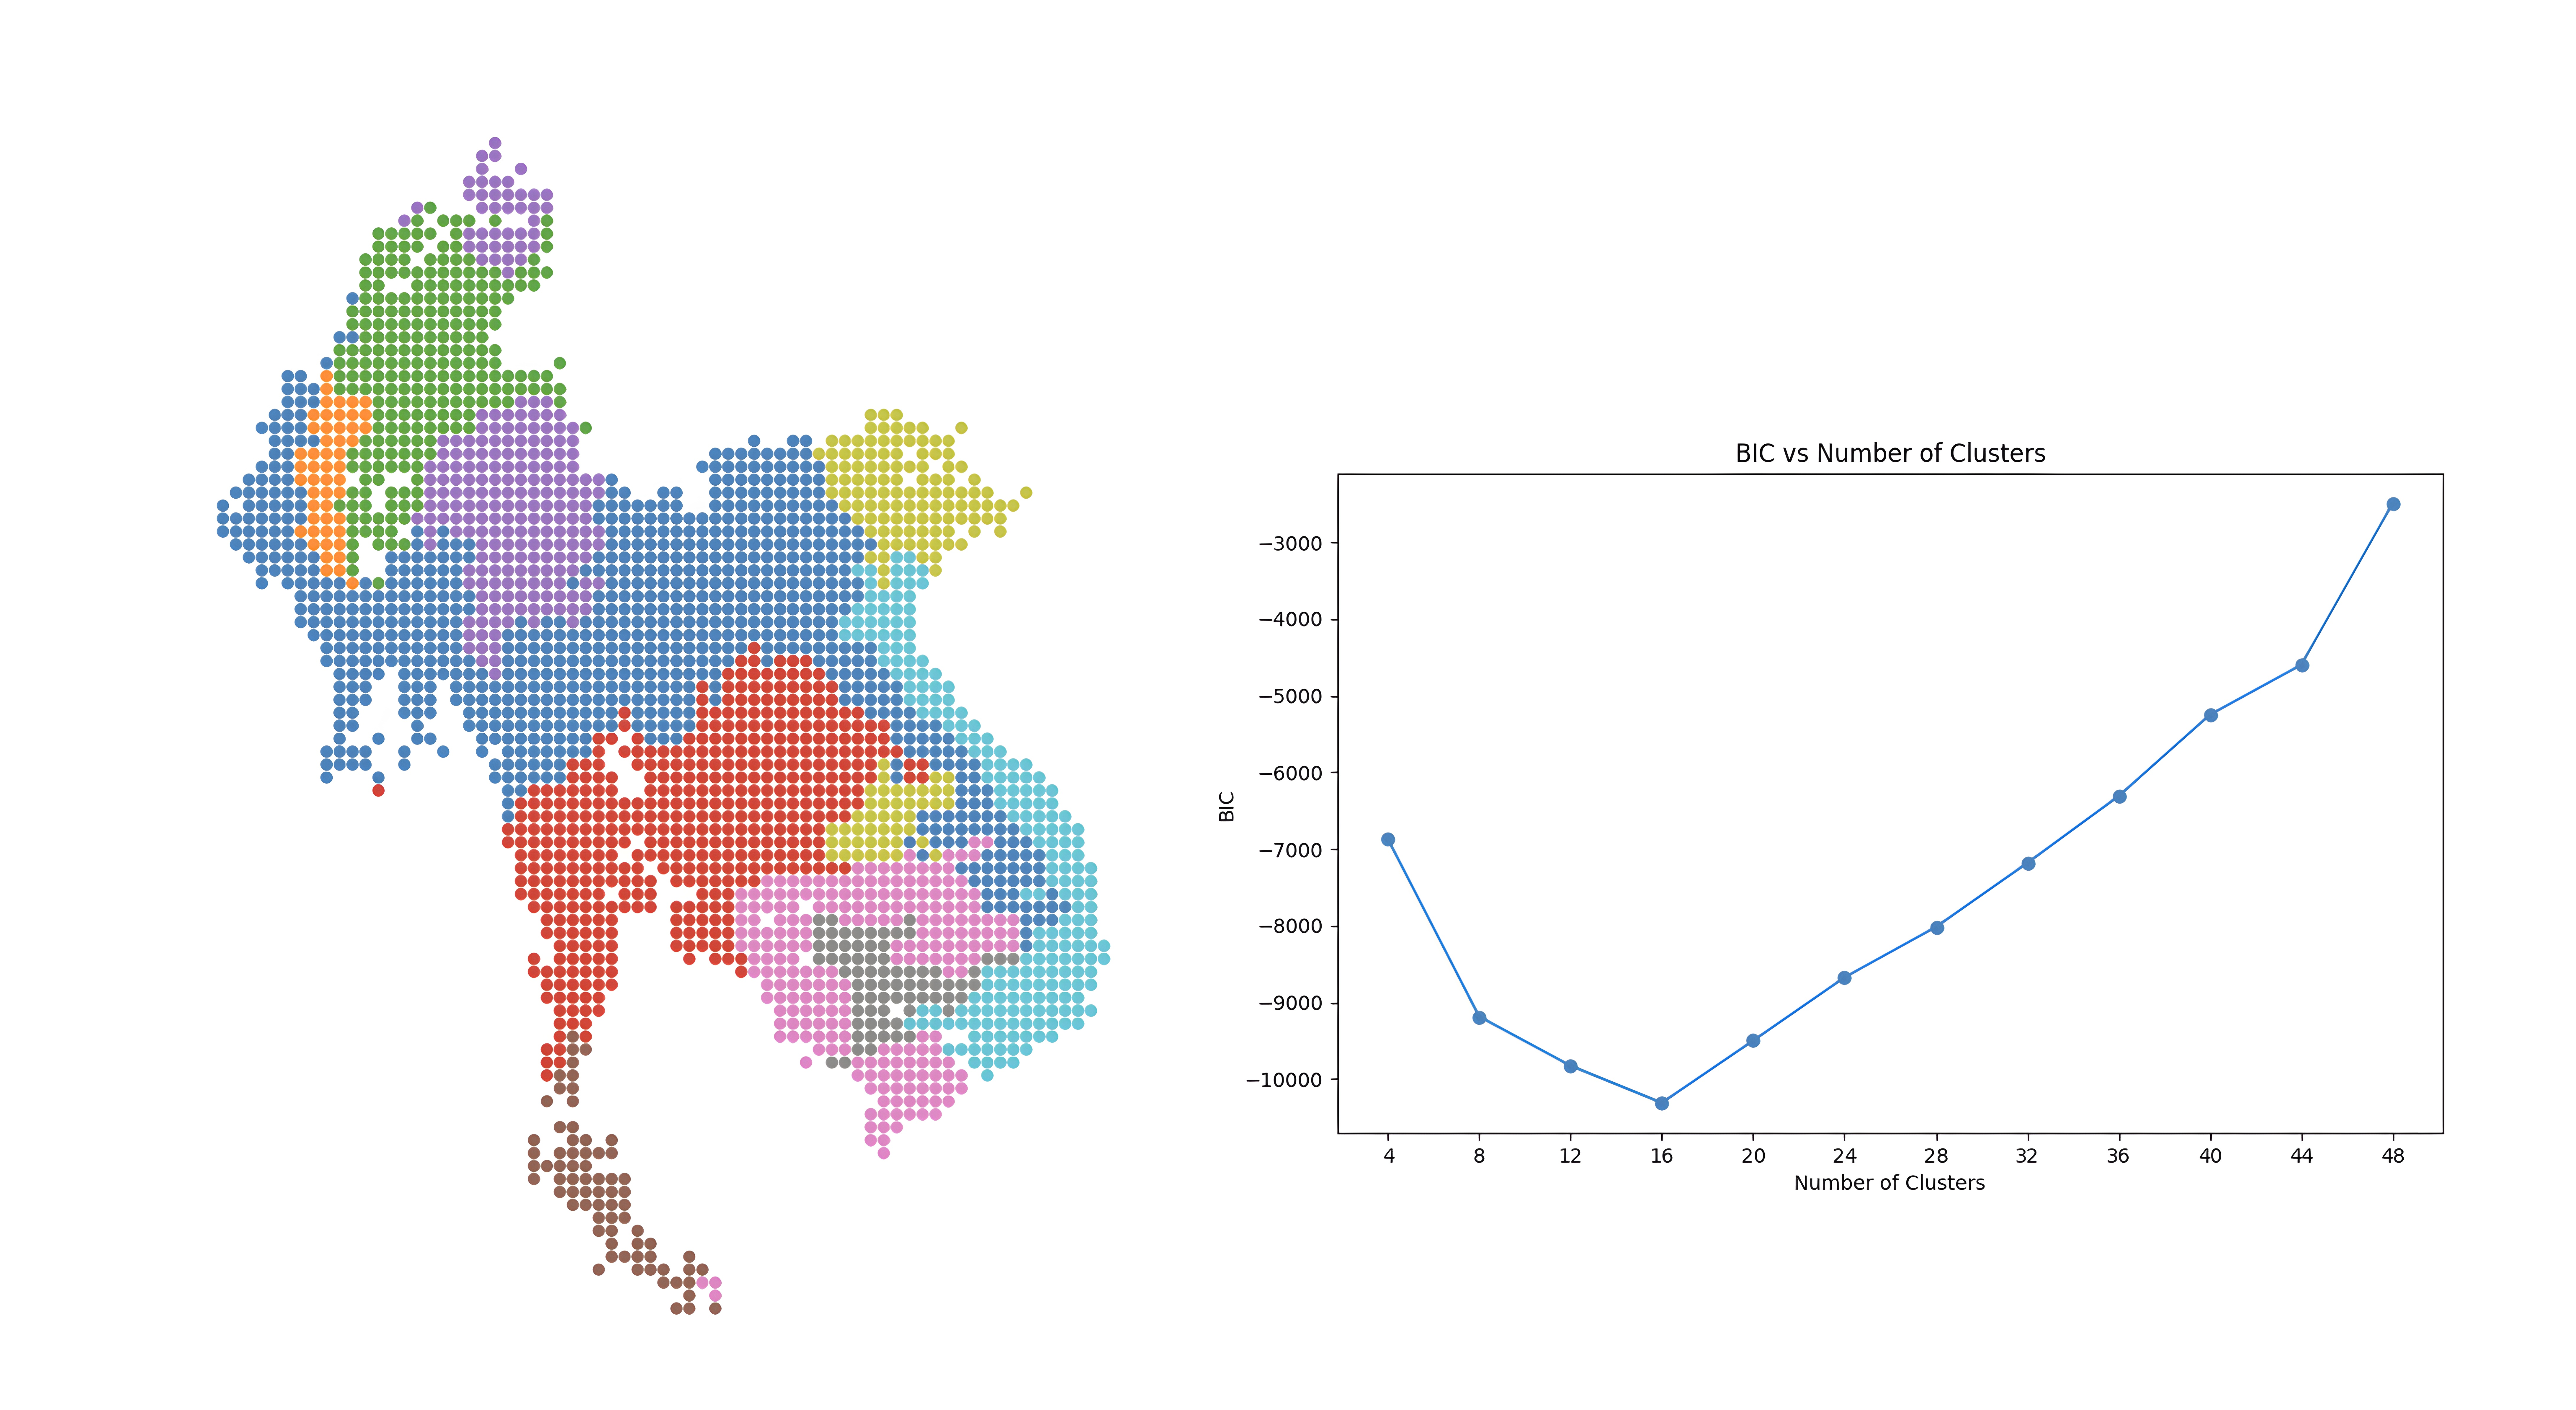
\includegraphics[width=0.8\textwidth]{./images/HQ_NewSKAnalysis.png}
\captionof{figure}{
{\fontfamily{lmss}\selectfont
Based on the lowest BIC score, 16 clusters were identified in the region. The VRC and Gap statistics are 250 and 1.74 respectively. Our clusters demonstrate that there is variability in fire patterns across SEA.
}
}
\end{center}
}%
%%%%%%%%%%%%%%%%%%%%%%%%%%%%%%%%%%%%%%%
%%%%%%%%%%%%%%%%%%%%%%%%%%%%%%%%%%%%%%%

\headerbox{Results on Fire-Rainfall Relationships}{name=rfr, column=1, row = 0}{
{\bf{\textsf{Generalized Additive Model}}}\\
{\fontfamily{lmss}\selectfont
\textbf{Model}: \textit{log(y) = s(MAP) + s(drought severity) + s(seasonality index) + s(PNV)}, where \textit{s} is the smooth function.
}
\begin{center}
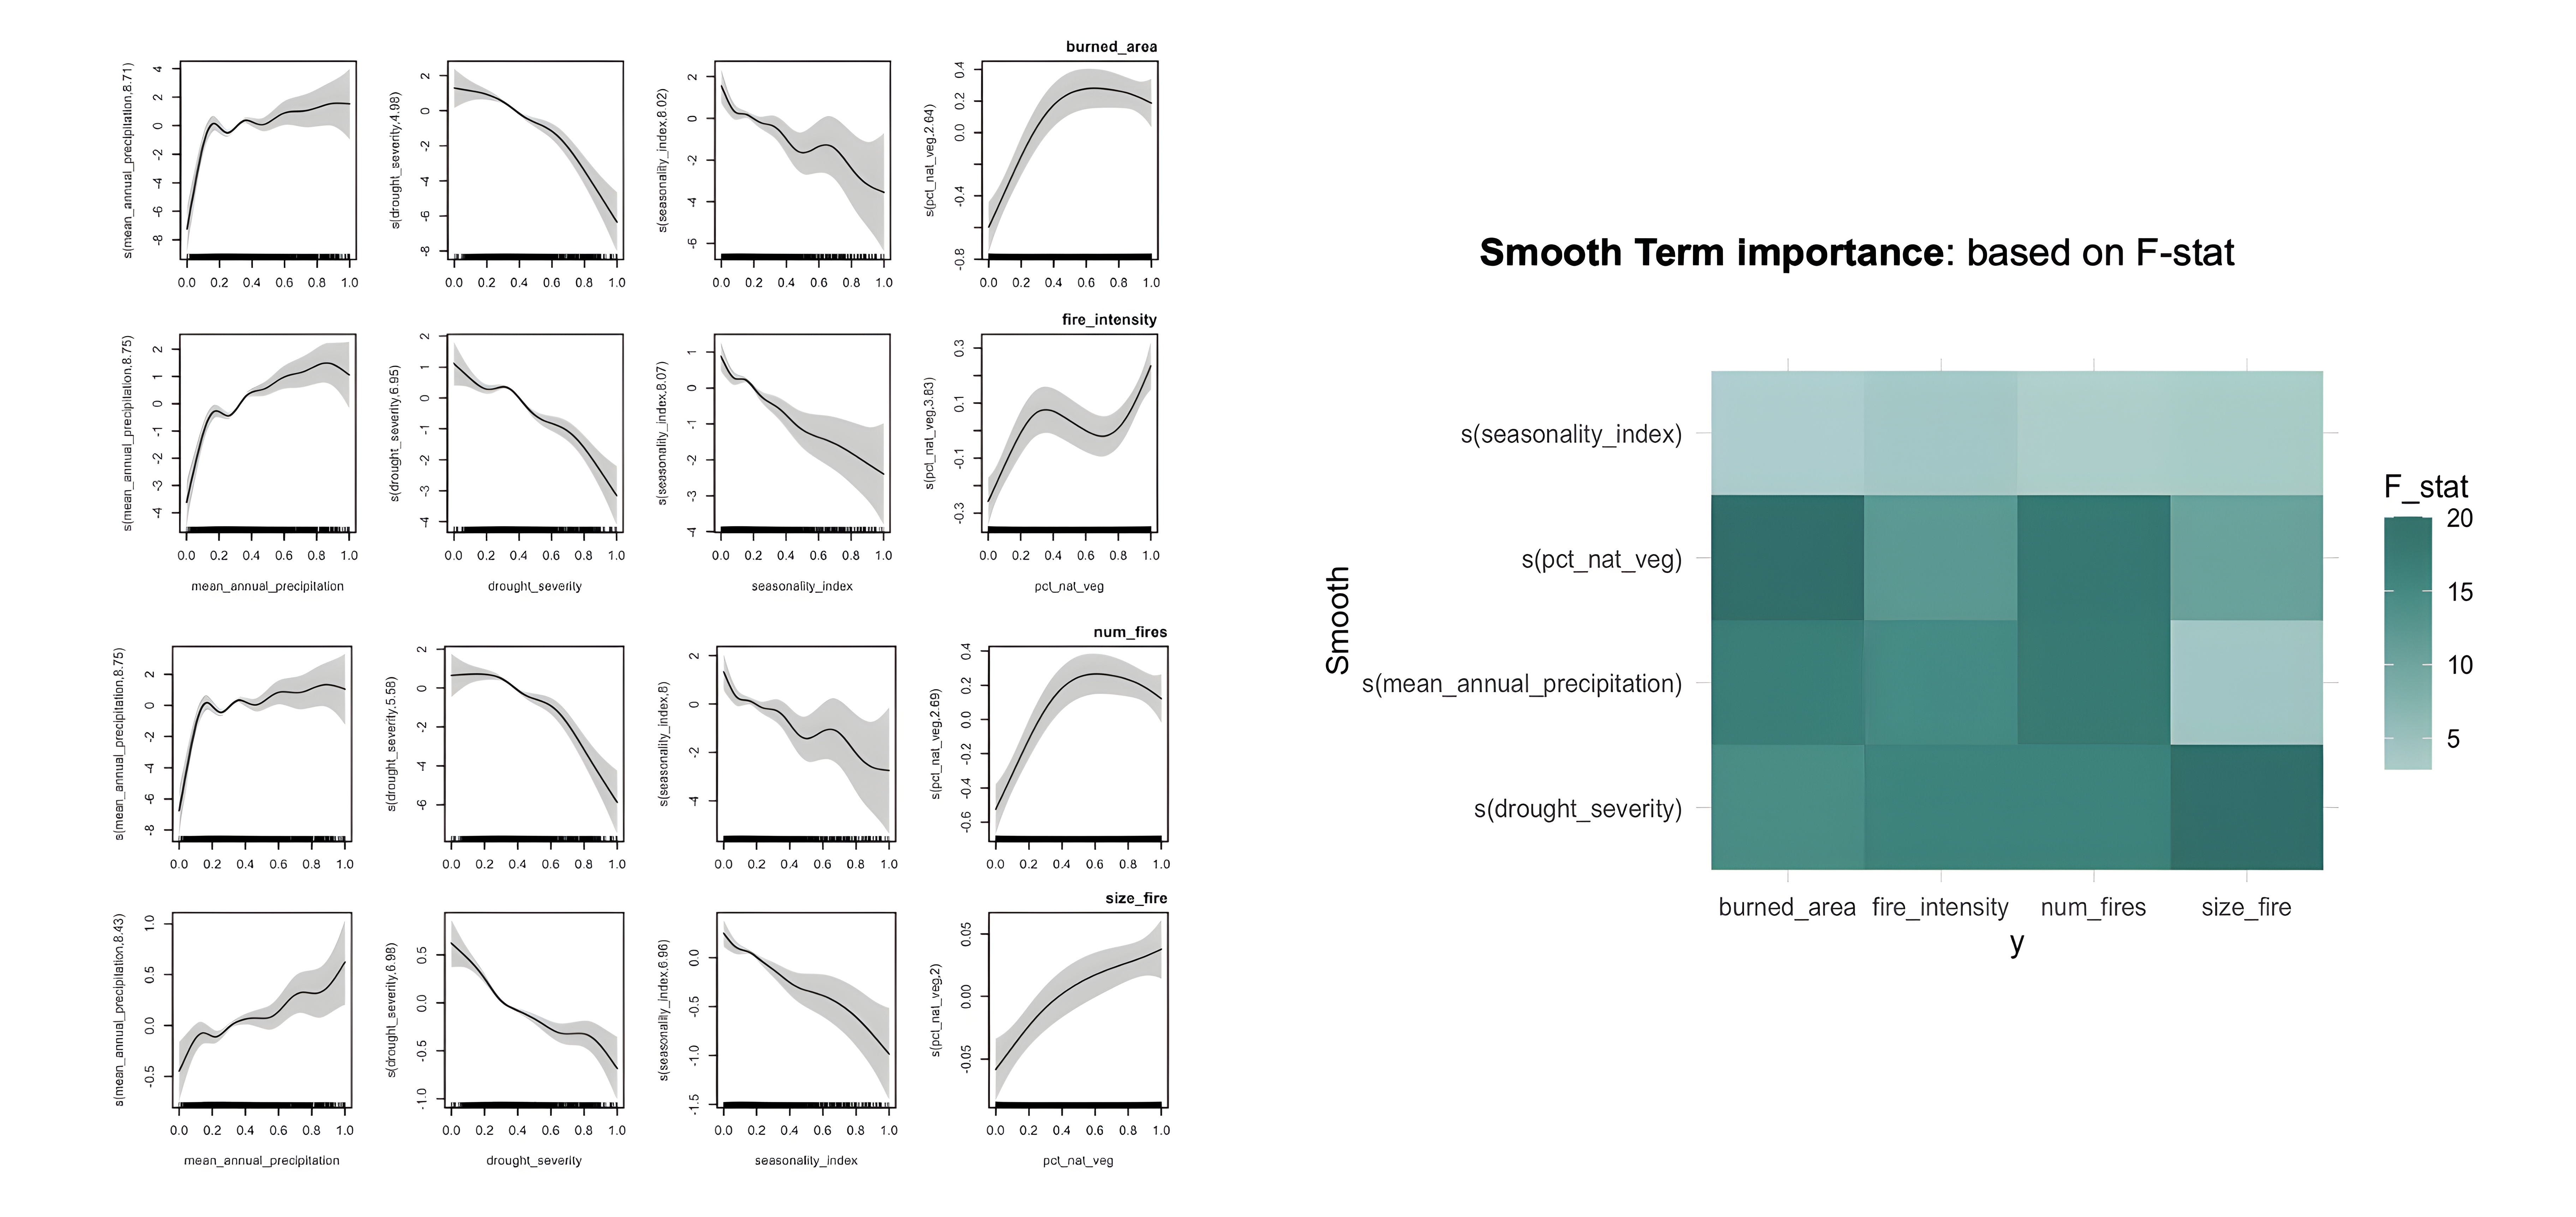
\includegraphics[width = 1.00\textwidth]{./images/HQ_GAMAll.png}
\captionof{figure}{
{\fontfamily{lmss}\selectfont
\textbf{Left}: Drought severity and Seasonality index appear to be negatively correlated with all fire variables. \textbf{Right}: Based on F-stat, drought severity seems to be most important in fire size model and percentage of natural vegetation seems to be most important in burned area and number of fires model. F-stat indicates whether the smooth function term for the variable is significant in a particular model.}
}
\end{center}

{\bf{\textsf{Random Forest Regression}}}\\
{\fontfamily{lmss}\selectfont
\textbf{Model}: \textit{log(y) = MAP + drought severity + seasonality index + PNV
}
}
\begin{center}
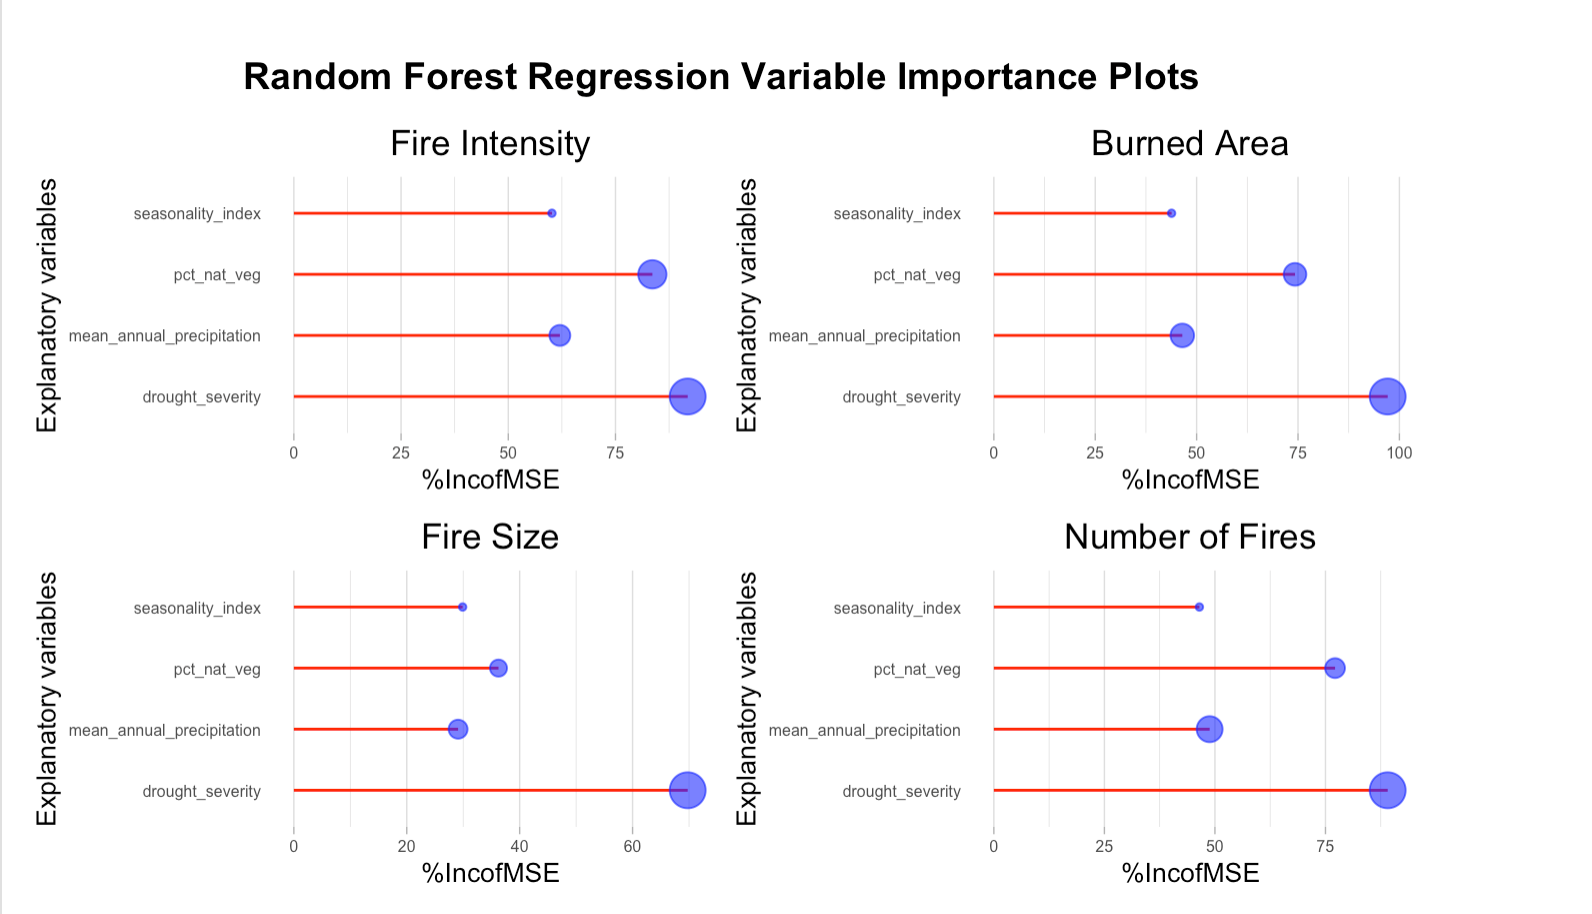
\includegraphics[width = 1.00\textwidth]{./images/VarImpPlot.png}
\captionof{figure}{
{\fontfamily{lmss}\selectfont
Variable Importance in Regression Model measured by percentage increase in mean square error (MSE). The metric percentage of increase in MSE indicates that how much MSE will the model increase after removing the corresponding explanatory variable. Drought Severity and Percentage of Natural Vegetation seem to be the most important variables in all four models. Seasonality index seems to be the least important here.}
}
\end{center}
}
%%%%%%%%%%%%%%%%%%%%%%%%%%%%%%%%%%%%%%%

\headerbox{Statistical Model Performance}{name=performance, column=2, row=0}{
{\bf{\textsf{Generalized Additive Model performance}}}
\vspace{-0.7em}
\begin{center}
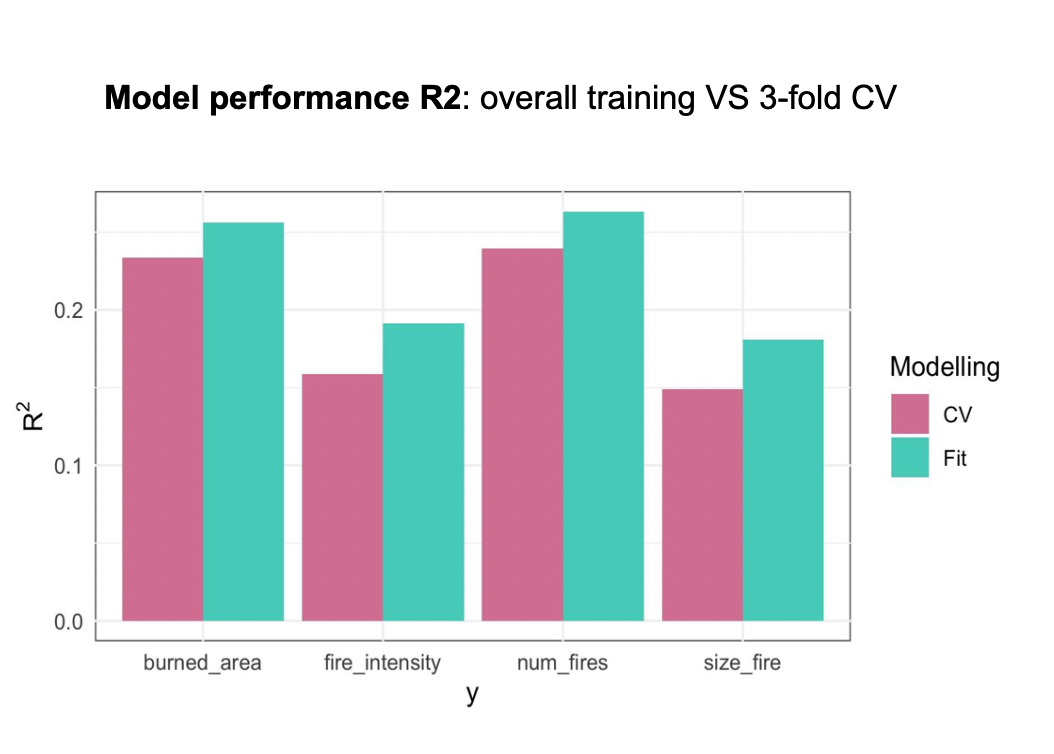
\includegraphics[width = 0.8\textwidth]{./images/GAMPerform.png}
\captionof{figure}{
{\fontfamily{lmss}\selectfont
Cross-validation and fit R-squared scores are relatively comparable. The R-squared values range around 0.15 to 0.28.}
}
\end{center}

{\bf{\textsf{Random Forest Regression performance}}}
\vspace{-0.7em}
\begin{center}
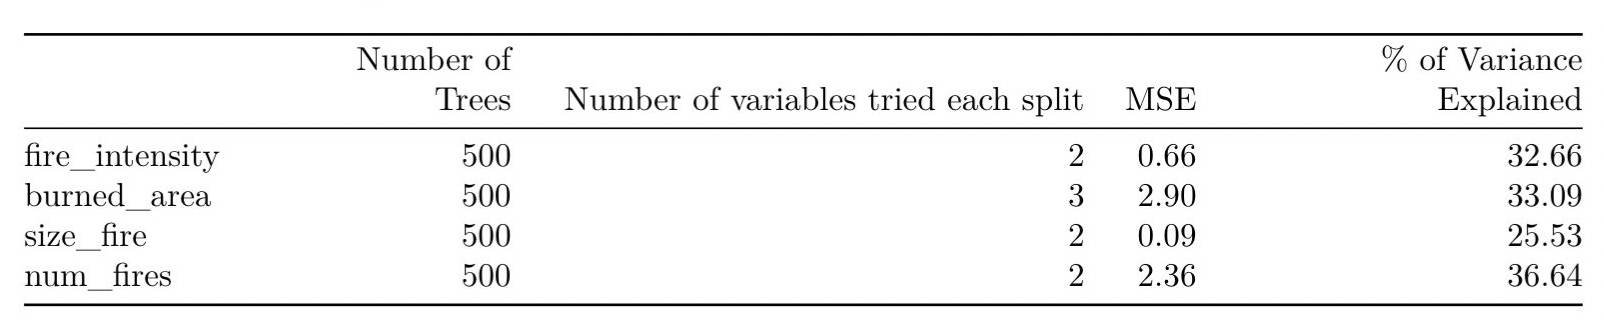
\includegraphics[width = \textwidth]{./images/RFPerform.png}
\captionof{figure}{
{\fontfamily{lmss}\selectfont
Hyperparameters for each model obtained from 3-fold cross-validation repeated 2 times. Relatively low MSE for fire intensity and fire size models. Percentage of variance explained ranges from 26-37\%.
}
}
\end{center}
}


\headerbox{Conclusions and Discussions}{name=conclusion,column=2, below=performance}{%
 {\bf{\textsf{Regionalization}}}
 \vspace{-0.7em}
 {\fontfamily{lmss}\selectfont
 \begin{flushitem}
    \item Our cluster metrics show there is a significant variability in fire patterns across SEA.
\end{flushitem}
}
 {\bf{\textsf{Rainfall Pattern Analysis}}}
 \vspace{-0.7em}
 {\fontfamily{lmss}\selectfont
 \begin{flushitem}
    \item Drought severity seems to have the greatest explanatory significance to the fire pattern data. 
    \item Both GAM and RF models agree on the direction of effect of mean annual precipitation, drought severity, and seasonality index.
\end{flushitem}
}
 {\bf{\textsf{Discussions}}}
 \vspace{-0.7em}
 {\fontfamily{lmss}\selectfont
 \begin{flushitem}
    \item Data is aggregated over 20-year average, hence, we have a rather low model performance/prediction score due to nature of data.
    \item Might also consider the correlation between rainfall patterns.
    \item Potentially capture non-linearity via polynomial regression while watching for overfitting.
\end{flushitem}
}
}
%%%%%%%%%%%%%%%%%%%%%%%%%%%%%%%%%%%%%%%%%%%%%%%%%%%%%%%%%%%%%%%%%%%%%%%%%%%%%%
%%%%%%%%%%%%%%%%%%%%%%%%%%%%%%%%%%%%%%%%%%%%%%%%%%%%%%%%%%%%%%%%%%%%%%%%%%%%%%%

%%%%%%%%%%%%%%%%%%%%%%%%%%%%%%%%%%%%%%%%%%%%%%%%%%%%%%%%%%%%%%%%%%%%%%%%%%%%%%%
%%%%%%%%%%%%%%%%%%%%%%%%%%%%%%%%%%%%%%%%%%%%%%%%%%%%%%%%%%%%%%%%%%%%%%%%%%%%%%
% \headerbox{Acknowledgements}{name=funding,column=1,span=1,below=rfr,above=bottom}{%
% %%%%%%%%%%%%%%%%%%%%%%%%%%%%%%%%%%%%%%%%%%%%%%%%%%%%%%%%%%%%%%%%%%%%%%%%%%%%%
% We would like to thank Professors \textbf{Keegan Korthauer}, \textbf{Melissa Lee}, and \textbf{Rodolfo Lourenzutti} for supervising the students involved in this project.
% }%
%%%%%%%%%%%%%%%%%%%%%%%%%%%%%%%%%%%%%%%%%%%%%%%%%%%%%%%%%%%%%%%%%%%%%%%%%%%%%
\end{poster}
\end{document}



% good work!